\centering
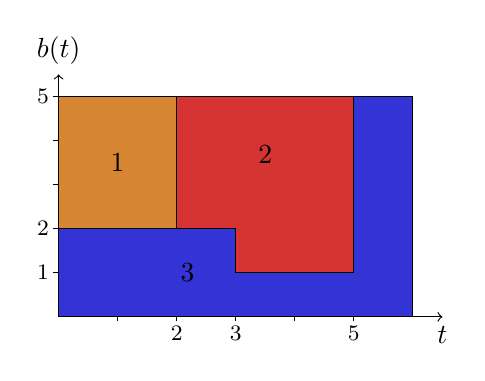
\begin{tikzpicture}
[xscale=0.75,yscale=0.56]
\node (O) at (0,0) {};
\draw[->] (0,0) -- (6.5,0) node[below] {$t$};
\draw[->] (0,0) -- (0,5.5) node[above] {$b(t)$};

\draw[fill=orange!80!black!80] (0,2) rectangle (2,5) node[midway] {$1$};
\path[draw,fill=blue!80!black!80] (0,0) -- (0,2) -- (3,2) -- (3,1) node[left=0.4cm] {$3$} -- (5,1) -- (5,5) -- (6,5)  -- (6,0) -- cycle;
\draw[fill=red!80!black!80] (2,5) -- (5,5) node[midway,below=0.5cm] {$2$} -- (5,1) -- (3,1) -- (3,2) -- (2,2) -- cycle;

\draw (0,1) node[left] {\footnotesize $1$};
\draw (0,2) node[left] {\footnotesize $2$};
\draw (0,5) node[left] {\footnotesize $5$};


\draw (2,0) node[below] {\footnotesize $2$};
\draw (3,0) node[below] {\footnotesize $3$};
\draw (5,0) node[below] {\footnotesize $5$};

\foreach \i in {1,...,5}{
\draw (\i,-0.1) -- (\i,0);
\draw (-0.1,\i) -- (0,\i);
}
\end{tikzpicture}
